% arara: xelatex: { shell: yes, synctex: yes }
%\RequirePackage[l2tabu, orthodox]{nag}
\documentclass[english,palatino]{ist-report}

\definecolor{bg}{rgb}{0.97,0.97,0.97}

% -- Bibliography
%\usepackage{csquotes}
%\usepackage{biblatex}
%\addbibresource{main.bib}

% -- Extra math options
\usepackage{mathtools}
\usepackage{siunitx} % Required for alignment
\sisetup{
  round-mode          = places, % Rounds numbers
  round-precision     = 2, % to 2 places
}

% -- Extra symbols
\usepackage{amssymb}
\usepackage{textcomp}
\usepackage{gensymb}
\usepackage{cancel}

% --  Image and float settings
\graphicspath{{graphics/}}
\usepackage{caption}
\usepackage{subcaption}
\usepackage{pdfpages}

% -- Graphs and diagrams
\usepackage{tikz}
\usepackage{pgfplots}
\usetikzlibrary{arrows.meta,positioning}
\pgfplotsset{compat=1.5, table/search path = {data}}

% -- Code listings
\usepackage{minted}
\setminted{linenos, bgcolor = bg, breaklines}
\setmintedinline{bgcolor = {}} 

% -- Extra table configs
\usepackage{booktabs}

\geometry{top=1.5cm}
\usepackage{todonotes}

\title{Integrated Avionic Systems}

\begin{document}

\thispagestyle{empty}

\begin{center}
	
\includegraphics[scale=0.3, trim = {93.4pt 219.7pt 77pt 221.9pt}]{IST_C_CMYK_POS}
	
	\vspace*{3mm}
	{\huge \textbf{Aircraft Altitude Control\\and Fault Processing}} \\
	\vspace*{4mm}
	{\large Control of an aircraft's altitude based on its sensor inputs and processing and mitigation of mid-flight system faults}
	\vspace*{4mm} \\
	\begin{tabular}{r l}
		Pedro \textsc{Afonso} & \textbf{66277} \\
		João \textsc{Manito} & \textbf{73096} \\
		Daniel \textsc{de Schiffart} & \textbf{81479}
	\end{tabular}
	
	\vspace*{3mm}
	{\Large \today}
	\vspace*{4mm} \\
	\rule{\linewidth}{0.5pt}
\end{center}

\begin{abstract}
	The objective of the second laboratory for this course was to control an aircraft's altitude and movement based on the input provided by its sensors and the transmission of data throughout the aircraft's onboard systems via its Local Area Network, characterizing the data protocols and preparing data for transmission. The second part of this laboratory had its focus more directed to the possibility of mid-flight faults to various aircraft systems, the handling of these faults and the simulation of data to maintain the control of the aircraft's altitude mentioned in the first part in the presence of faults in any of the crucial systems for this process. The work was to be implemented in C code for the major part of its simulations, with an initial theoretical segment being done with the use of \textsc{MATLAB} to obtain fixed results relevant to the work.
\end{abstract}

{\hypersetup{linkcolor = black} \tableofcontents}

\part{Aircraft Altitude Sensor and On-Board Data Bus}

This first part of the report focuses on the gathering of external data, in this case the pressure, through the on-board sensors, modelling of sensor behaviour using gathered data, and the comparison of this theoretical model with the actual data to study the error obtained. This work is followed by the study of the transmission of data through the aircraft's on-board system local network.

\section{Modeling The Input Data}

For this first section, we were provided a set of gathered voltage data from a sensor at three different temperatures, with each voltage value accompanied by the corresponding static pressure value. In total, a total of 219 lines of data, which means voltage values for 219 different real static pressure values. A sample of the data provided is seen in table \ref{tab:datain}.

\begin{table}[ht]
	\centering
	\resizebox{\textwidth}{!}{
	\begin{tabular}{c|c|c|c}\toprule
		Pressure [mbar]		& Output [Volt] at $-45\degree C$	& Output [Volt] at $25\degree C$		& Output [Volt] at $125\degree C$	\\
		\midrule
		\num{1.0000000e+01}	& \num{9.6891912e-02}				& \num{3.9214138e-02}					& \num{8.0487284e-02}				\\
		$\vdots$			& $\vdots$							& $\vdots$								& $\vdots$							\\
		\bottomrule
	\end{tabular}}
	\caption{Example of the provided data formatting.}
	\label{tab:datain}
\end{table}

The data was to be used to determine a model for the pressure, using the voltage and ambient temperature as model inputs. For this purpose, we used MATLAB's \href{https://www.mathworks.com/help/curvefit/fit.html}{\texttt{fit}} function from the \textit{Curve Fitting Toolbox}, using a second order polynomial for the temperature axis and a fourth-order polynomial curve for the voltage fitting. This yielded the polynomials found in equation \ref{eq:fitpoly}.

\begin{gather}\label{eq:fitpoly}
	%p(v,T) = 27.21 + 311.6v + 0.05789T - 20.33v^2 + 0.1015vT
	\begin{split}
		p(v,T) = 5.639 + 382.1v - 0.05732T - 69.73v^2 + 0.2646vT + 0.0002634T^2 + 11.53v^3 \\ - 0.05126v^2T - 0.0002063vT^2 - 0.8314v^4 + 0.004329v^3T + 4.644\times10^{-5}v^2T^2
	\end{split}
\end{gather}

The model was plotted against the provided input data and can be found in figure \ref{fig:3dplotmain} in page \pageref{fig:3dplotmain}. The raw data from the MATLAB output can be found below.  

\begin{minted}{text}
Linear model Poly42:
     sf(x,y) = p00 + p10*x + p01*y + p20*x^2 + p11*x*y + p02*y^2 + p30*x^3 + 
                    p21*x^2*y + p12*x*y^2 + p40*x^4 + p31*x^3*y + p22*x^2*y^2
     Coefficients (with 95% confidence bounds):
       p00 =       5.639  (1.566, 9.713)
       p10 =       382.1  (371.3, 392.9)
       p01 =    -0.05732  (-0.1234, 0.008728)
       p20 =      -69.73  (-78.75, -60.72)
       p11 =      0.2646  (0.166, 0.3632)
       p02 =   0.0002634  (-0.0003534, 0.0008803)
       p30 =       11.53  (8.749, 14.31)
       p21 =    -0.05126  (-0.0942, -0.008322)
       p12 =  -0.0002063  (-0.0008547, 0.0004422)
       p40 =     -0.8314  (-1.113, -0.5502)
       p31 =    0.004329  (-0.001359, 0.01002)
       p22 =   4.644e-05  (-8.942e-05, 0.0001823)
\end{minted}

\section{ARINC Data Bus Sketching}

For this question we considered the range of values between $\num{-45}\degree C$ and $\num{125}\degree C$, which leaves us with a total of 170 values of temperature to be transmitted. With an additional request of an accuracy of $\num{0.1}\degree C$, we need ten times as many values. All things considered, we need to transmit any values in a range of 1700 possibilities. Going through the amount of possible values held by a number of binary bits, we look for the amount of bits to meet this requirement.

\begin{table}[ht]
	\centering
	\begin{tabular}{ccc}
		\vdots		& $=$	& \vdots	\\
		$2^9$		& $=$	& $512$		\\
		$2^{10}$	& $=$	& $1024$	\\
		$2^{11}$	& $=$	& $2048$	\\
		$2^{12}$	& $=$	& $4096$	\\
		\vdots		& $=$	& \vdots	\\
	\end{tabular}
\end{table}

With this in mind, and considering using an offset of values to eliminate the need for a signal bit (or even converting the temperature to Kelvin), we need at the very least 11 bits to transmit.

\begin{figure}[ht]
	\centering
	%\resizebox{\textwidth}{!}{
	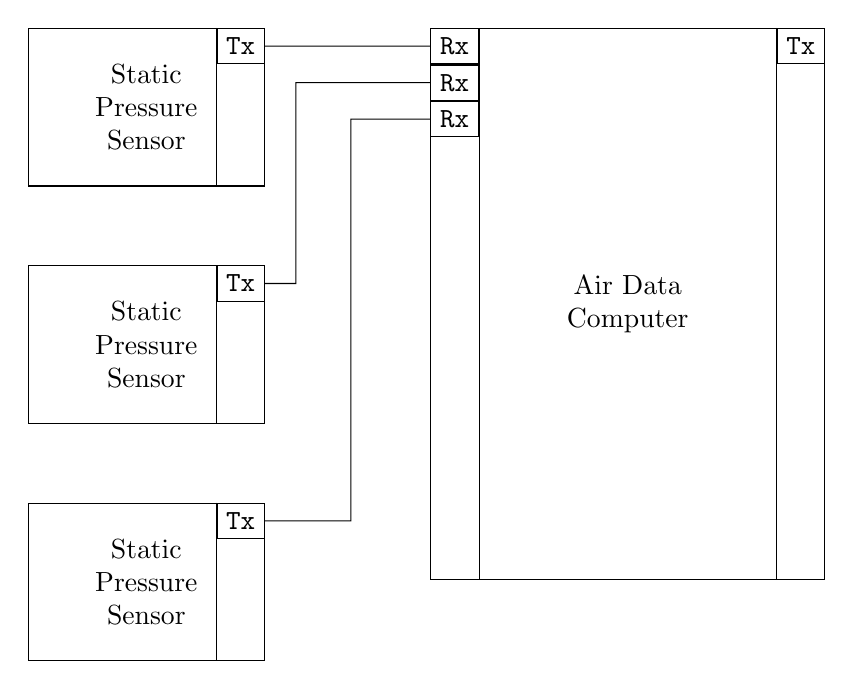
\begin{tikzpicture}[scale=0.7]
		\node (sp1) at (0,0) [rectangle, draw, align=center,minimum width = 3cm, minimum height = 2cm] {Static \\ Pressure \\ Sensor};
		\node (tx11) at (sp1.north east) [rectangle,draw,anchor = north east] {\texttt{Tx}};
		\path [draw,very thin] (tx11.north west) -- (tx11.north west|-sp1.south);
		\node (sp2) [below=of sp1,rectangle, draw, align=center,minimum width = 3cm, minimum height = 2cm] {Static \\ Pressure \\ Sensor};
		\node (tx21) at (sp2.north east) [rectangle,draw,anchor = north east] {\texttt{Tx}};
		\path [draw,very thin] (tx21.north west) -- (tx21.north west|-sp2.south);
		\node (sp3) [below=of sp2,rectangle, draw, align=center,minimum width = 3cm, minimum height = 2cm] {Static \\ Pressure \\ Sensor};
		\node (tx31) at (sp3.north east) [rectangle,draw,anchor = north east] {\texttt{Tx}};
		\path [draw,very thin] (tx31.north west) -- (tx31.north west|-sp3.south);
		\path (sp1.north east) ++(3,0) node (adc) [anchor = north west, rectangle, draw, align=center, minimum width = 5cm, minimum height = 7cm] {Air Data \\ Computer};
		\node (rxa1) at (adc.north west) [rectangle,draw,anchor = north west] {\texttt{Rx}};
		\path [draw,very thin] (rxa1.north east) -- (rxa1.north east|-adc.south);
		\node (rxa2) at (rxa1.south west) [rectangle,draw,anchor = north west] {\texttt{Rx}};
		\node (rxa3) at (rxa2.south west) [rectangle,draw,anchor = north west] {\texttt{Rx}};
		\node (txa1) at (adc.north east) [rectangle,draw,anchor = north east] {\texttt{Tx}};
		\path [draw,very thin] (txa1.north west) -- (txa1.north west|-adc.south);
		\path [draw] (tx11) -- (rxa1);
		\path [draw] (tx21)  -- ++(1,0) coordinate (c1) -- (c1|-rxa2) -- (rxa2);
		\path [draw] (tx31)  -- ++(2,0) coordinate (c2) -- (c2|-rxa3) -- (rxa3);
	\end{tikzpicture}
	%}
	\caption{Air Data Computer.}
	\label{fig:adc}
\end{figure}

\begin{gather*}
	h(p) = 145366.45\left(1 - \left(\frac{p_s}{1013.25}\right)^{0.190284}\right)
\end{gather*}

\part{Dealing With Faults and Errors}

\begin{align*}
	\dot{x} &= v\cos\gamma + at\cos(\gamma + \alpha) \\
	\dot{h} &= v\sin\gamma + at\cos(\gamma + \alpha) \\
	x &= \dot{x}t \\
	h &= \dot{h}t \\
	\tan\gamma &= \frac{\dot{x}}{\dot{h}}
\end{align*}
\begin{gather*}
	v = at \\
	a \propto T \\
\end{gather*}

\section{Possible Faults}

Within the simple system implemented in this laboratory, several components can fail or behave unexpectedly. Whether it's the control system or the sensors used, either one can have a fault at some point and the control system needs to be ready to return the control to the pilot should a fault be detected somewhere.

This fault detection will be done by monitoring the flight variables and their behaviour throughout the simulation. The first step should then be define what constitutes a fault. By definition,
\begin{quote} \itshape
	A fault is a deviation (of a feature) from the acceptable, standard operational condition.
\end{quote}
For sensors, we can consider four types of faults, either sensor bias, drift, loss of accuracy or freeze. The sources for these faults come from either the barometric sensor or the temperature A/D conversion and data transmission.

\listoftodos

\pagebreak
\appendix

\section{Data Plots}

\begin{figure}[ht]
	\centering
	\begin{tikzpicture}
		\begin{axis}[domain=0:5,y domain=-45:125,view={-30}{25},xlabel=$\si{\volt}$,ylabel=$\degree C$, zlabel=$\si{\pascal}$,width=0.7\textwidth]
			\addplot3[surf,samples=05] {5.639 + 382.1 * x - 0.05732 * y - 69.73 * x^2 + 0.2646 * x * y + 0.0002634 * y^2 + 11.53 * x^3 - 0.05126 * x^2 * y - 0.0002063 * x * y^2 - 0.8314 * x^4 + 0.004329 * x^3 * y + 4.644 * 0.00001 * x^2 * y^2};
			\addplot3[only marks,color=red,mark=o] table [x index = {1}, z index = {0}, y expr = -45, col sep = comma] {inputdata.csv};
			\addplot3[only marks,color=blue,mark=o] table [x index = {2}, z index = {0}, y expr = 25, col sep = comma] {inputdata.csv};
			\addplot3[only marks,color=green,mark=o] table [x index = {3}, z index = {0}, y expr = 125, col sep = comma] {inputdata.csv};
		\end{axis}
	\end{tikzpicture}
	\caption{Comparison of the data provided and the modelled polynomial.}
	\label{fig:3dplotmain}
\end{figure}

\begin{figure}[ht]
	\centering
	\begin{tikzpicture}
		\begin{axis}[domain=0:5,xlabel=\si{\volt},ylabel=\si{\pascal},width=0.7\textwidth]
			\addplot table [col sep = comma, x index = {1}, y index = {0}] {inputdata.csv};
			\addplot table [col sep = comma, x index = {2}, y index = {0}] {inputdata.csv};
			\addplot table [col sep = comma, x index = {3}, y index = {0}] {inputdata.csv};
			\addplot [mark=none,mark size = 1pt] {5.639 + 382.1 * x - 0.05732 * (-45) - 69.73 * x^2 + 0.2646 * x * (-45) + 0.0002634 * (-45)^2 + 11.53 * x^3 - 0.05126 * x^2 * (-45) - 0.0002063 * x * (-45)^2 - 0.8314 * x^4 + 0.004329 * x^3 * (-45) + 4.644 * 0.00001 * x^2 * (-45)^2};
			\addplot [mark=none, mark size = 1pt] {5.639 + 382.1 * x - 0.05732 * 25 - 69.73 * x^2 + 0.2646 * x * 25 + 0.0002634 * 25^2 + 11.53 * x^3 - 0.05126 * x^2 * 25 - 0.0002063 * x * 25^2 - 0.8314 * x^4 + 0.004329 * x^3 * 25 + 4.644 * 0.00001 * x^2 * 25^2};
			\addplot [mark=none, mark size = 1pt] {5.639 + 382.1 * x - 0.05732 * 125 - 69.73 * x^2 + 0.2646 * x * 125 + 0.0002634 * 125^2 + 11.53 * x^3 - 0.05126 * x^2 * 125 - 0.0002063 * x * 125^2 - 0.8314 * x^4 + 0.004329 * x^3 * 125 + 4.644 * 0.00001 * x^2 * 125^2};
		\end{axis}
	\end{tikzpicture}
	\caption{Side-view of the plots versus the modeled version at the same temperature.}
	\label{fig:2dplotmain}
\end{figure}

\end{document}
